%%% use twocolumn and 10pt options with the asme2e format
\documentclass[twocolumn,10pt]{asme2e}
\special{papersize=8.5in,11in}
\usepackage{graphicx}
\usepackage{caption}
\usepackage{subcaption}
\usepackage{lipsum}
\usepackage{amsmath}
\usepackage{multicol}

\confshortname{FEDSM 2020}
\conffullname{the ASME 2020 Fluids Engineering Division Summer Meeting}

\confdate{July 12-16}
\confyear{2020}
\confcity{Orlando, Florida}
\confcountry{USA}

\papernum{FEDSM2020-12388}

%%% You need to remove 'DRAFT: ' in the title for the final submitted version.
\title{DRAFT: The Effect of Variying Viscosity in Turbulent Channel Flow}


%%% first author
\author{Victor Coppo Leite
    \affiliation{
	Ken and Mary Alice Lindquist\\Department of Nuclear Engineering\\
	Pennsylvania State University\\
	State College, PA 16801\\
    Email: vbc5085@psu.edu
    }	
}

%%% second author
%%% remove the following entry for single author papers
\author{Elia Merzari
    \affiliation{
	Ken and Mary Alice Lindquist\\Department of Nuclear Engineering\\
	Pennsylvania State University\\
	State College, PA 16801\\
    Email: ebm5153@psu.edu
    }	
}

\begin{document}

\maketitle    

%%%%%%%%%%%%%%%%%%%%%%%%%%%%%%%%%%%%%%%%%%%%%%%%%%%%%%%%%%%%%%%%%%%%%%
\begin{abstract}
{\it In various applications in nuclear engineering and in particular in test reactors, heat removal is carried by single-phase axial flow. In these applications, we observe sharp changes in molecular viscosity while the density presents very limited changes. As a consequence, the Reynolds number increases often by 2-3 folds across the channel, with an inlet value often transitional.  In these conditions, turbulence changes significantly across the length of the channel with redistribution and thinning of the boundary layers. This is different from acceleration as the effect of changes in density is negligible. We aim to characterize in detail this phenomenon. 

In particular Nek5000, a spectral-element computational fluid dynamics (CFD) code, will be used to perform DNS of fluid flow in the transition regime for channel flow with varying viscosity.  We set up a novel benchmark case: the channel is extended in the stream-wise direction up to 20pi. The viscosity is kept constant in the first 4pi region. This inlet region is used as a cyclic region to obtain a fully developed flow profile at the beginning of the ramping region. The ramping region (4pi -20pi) is defined as a transition region where the viscosity is linearly decreased along the channel. The flow is homogenous in the span-wise direction due to the periodic boundary conditions. Due to the cyclic and wall boundary conditions, the flow is non-homogenous in the stream-wise and wall-normal direction respectively.

In this study, specific focusS is given to the investigation of turbulence properties and structures in the near-wall region along the flow direction. Detailed turbulence budgets are collected and investigated. As expected, the results show that variation in the Reynolds across a channel does not cause an immediate change in the size of turbulent structures in the ramp region and a delay is in fact observed. Moreover, the results from the present study are compared with a correlation available in the literature for the friction velocity and as a function of the Reynolds-number.}
\end{abstract}

%%%%%%%%%%%%%%%%%%%%%%%%%%%%%%%%%%%%%%%%%%%%%%%%%%%%%%%%%%%%%%%%%%%%%%
\begin{nomenclature}
\entry{$a$}{Viscosity linear coefficient.}
\entry{$C$}{Contractioning parameter.}
\entry{${F_{Ci}}$}{Delayed function of Cases ${i}$=I,II and III.}
\entry{$R$}{Relaxing parameter.}
\entry{$Re$}{Reynolds number.}
\entry{$Re_{\tau}$}{Friction Reynolds number.}
\entry{$u_{\tau}$}{Friction velocity.}
\entry{$x$}{Streamwise direction.}
\entry{$y$}{Vertical direction.}
\entry{$z$}{Spanwise direction.}
\entry{$\delta$}{Height of the turbulence channel.}
\entry{${\delta}_{i}$}{Streamwise position where Region $i$ starts, ${i}$=I,II and III.}
\entry{${\Lambda}$}{Signal contribution in the delayed function.}
\entry{$\nu$}{Viscosity.}
\entry{${\tau}_w$}{Shear stress at the wall.}
\end{nomenclature}


%%%%%%%%%%%%%%%%%%%%%%%%%%%%%%%%%%%%%%%%%%%%%%%%%%%%%%%%%%%%%%%%%%%%%%
\section*{INTRODUCTION}

A schematic of the turbulence channels simulated are shown in Fig.~\ref{fig:geometry_turbchannel}. In this figure, Regions I, II and III are defined by two planes crossing the channel. A cycling region is implemented within Region I, Fig.~\ref{fig:cycling_region}.
In this problem, the viscosity \(\nu\) is a function of \(x\), i.e., the streamwise distance. This parameter has constants values of \(1E-4\) Pa.s and \(5E-5\) Pa.s along Regions I and III respectively, while in region II it decreases with respect to the inverse of \(x\).

In the present work, three cases varying the length of Region II are studied. Cases I, II and III have their Region II length of respectively \(16\pi\), \(8\pi\) and \(4\pi\). Fig.~\ref{fig:viscosity} shows the plot of the viscosity as a function of \(x\) for each one of these cases and Fig.~\ref{fig:reynolds} shows the plot of the Reynolds number for them.

For all three Cases the inleat flow in Region I is considered to be fully developed with \(Re_{\tau}=550\), i.e., the same conditions as in \cite{hoyas2008}. Periodic condition is considered for the boundaries of the spamwise direction, i.e., \(z\) axis, and finally wall conditions are considered for the boudaries of the vertical direction, i.e., \(y\) axis.

\begin{figure}[t]
	\centering
	\scalebox{0.5}
	{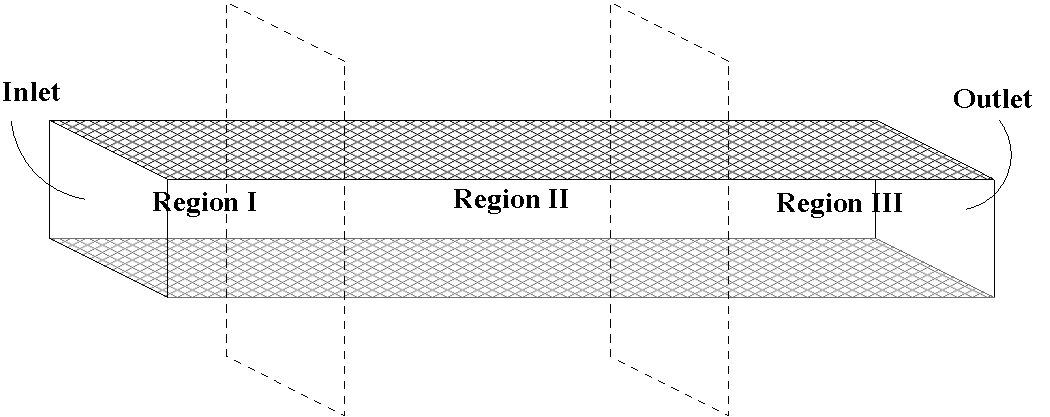
\includegraphics{geometry_turbchannel.pdf}}
	\scalebox{0.4}
	{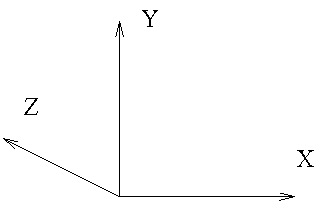
\includegraphics{axis.pdf}}
	\caption{Geometry of the turbulence channel, the channel is divided into three different Regions.}
	\label{fig:geometry_turbchannel}
	\end{figure}

\begin{figure}[t]
	\centering
	\scalebox{0.5}
	{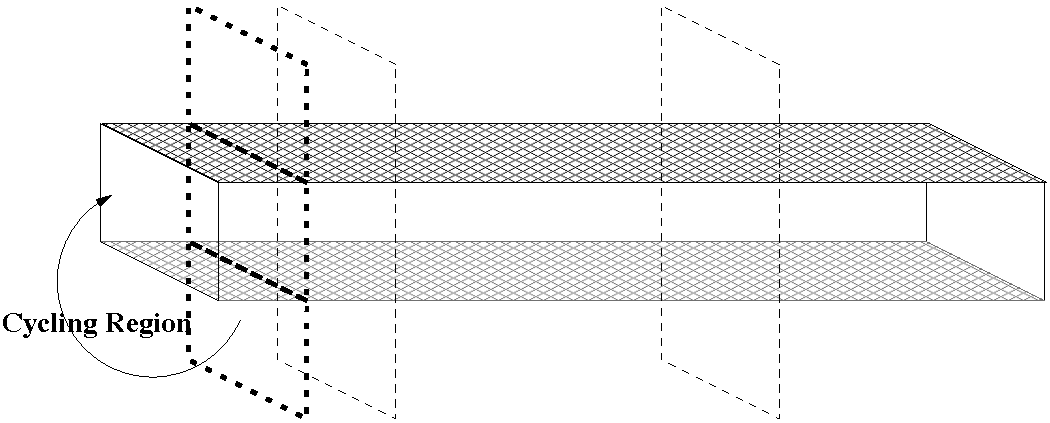
\includegraphics{cycling_region.pdf}}
	\caption{Cyclic region in the inlet.}
	\label{fig:cycling_region}
\end{figure}

\begin{figure}[t]
	\centering
	\scalebox{0.5}
	{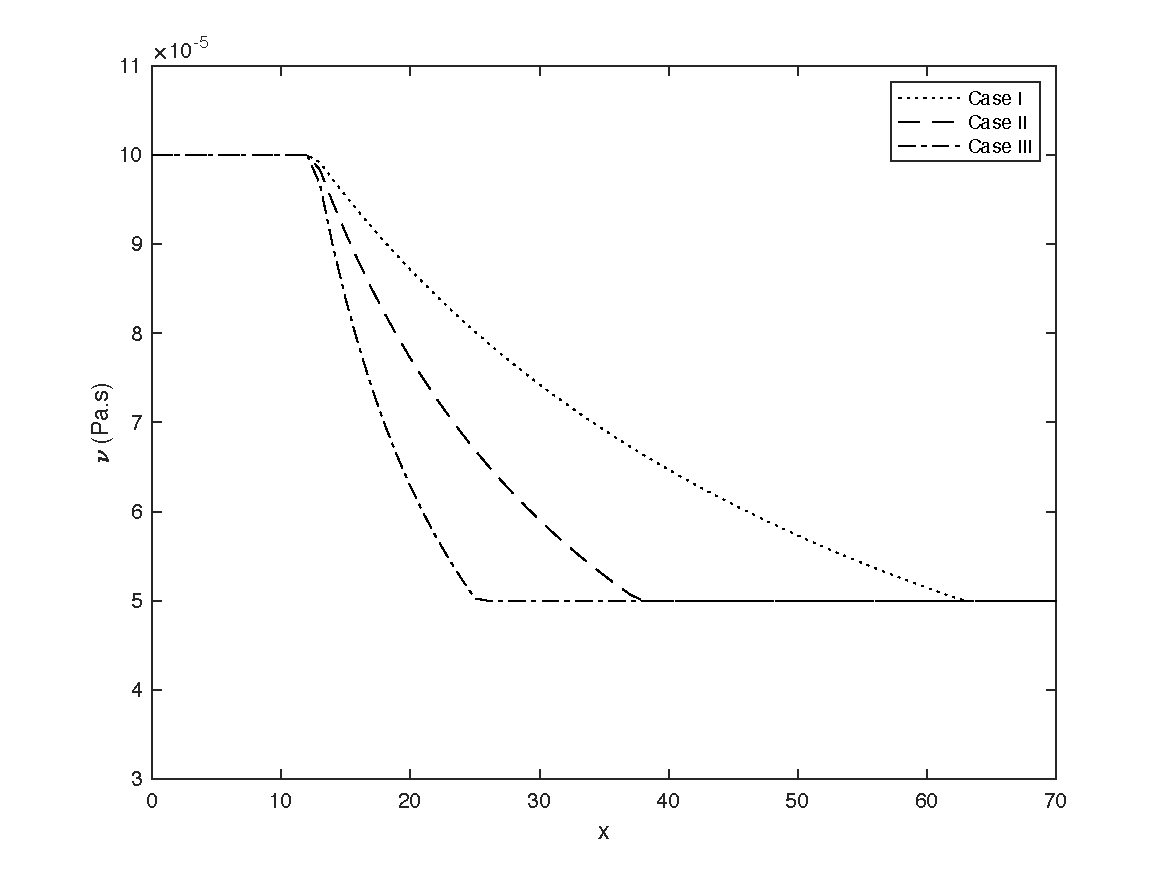
\includegraphics{viscosity.pdf}}
	\caption{The viscosity of the considered Cases as a function of \(x\).}
	\label{fig:viscosity}
	\end{figure}

\begin{figure}[t]
	\centering
	\scalebox{0.5}
	{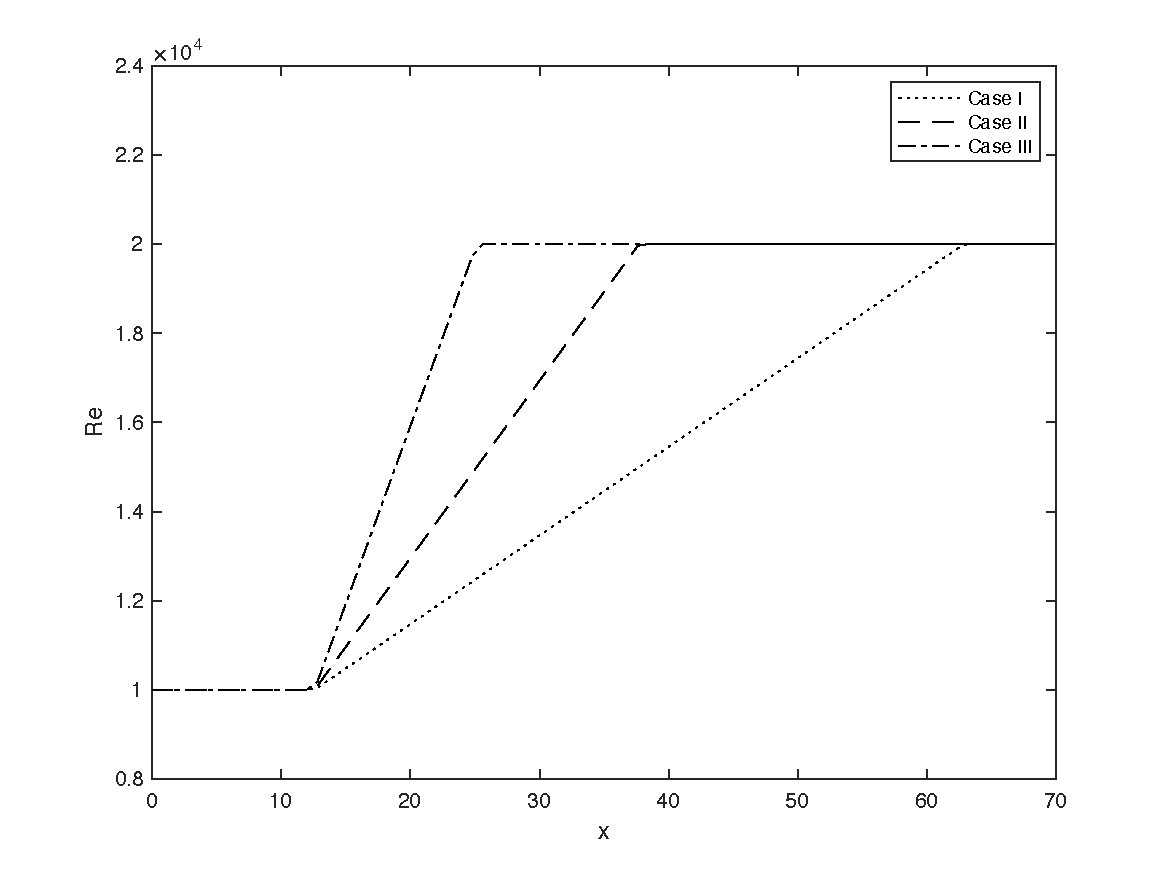
\includegraphics{reynolds.pdf}}
	\caption{The Reynolds number as a function of the \(x\) for the considered Cases.}
	\label{fig:reynolds}
\end{figure}

%%%%%%%%%%%%%%%%%%%%%%%%%%%%%%%%%%%%%%%%%%%%%%%%%%%%%%%%%%%%%%%%%%%%%%
\section*{METHODS - DIRECT NUMERICAL SIMULATION}

In order to resolve the finest turbulent scales, the calculations of this work has been developed through Direct Numerical Simulation (DNS). To do so Nek5000 was employed, a spectral element code developed in Argonne National Laboratory (ANL). Nek5000 has been validated in references \cite{merzari2013} and \cite{Obabko2011}.

The solution of this method is given by trigonometric series, in each element a polynomial functions of up to the twelveth degree have been employed to discretize the velocity field. Fig.~\ref{fig:mesh} shows an example of the grid from half of the channel's cross section. One should notice that the discretization presented by this particular area is identical through all model's domain and it is only presented half of the cross-section for better visualization of the frame.

\begin{figure}[t]
	\centering
	\scalebox{0.16}
	{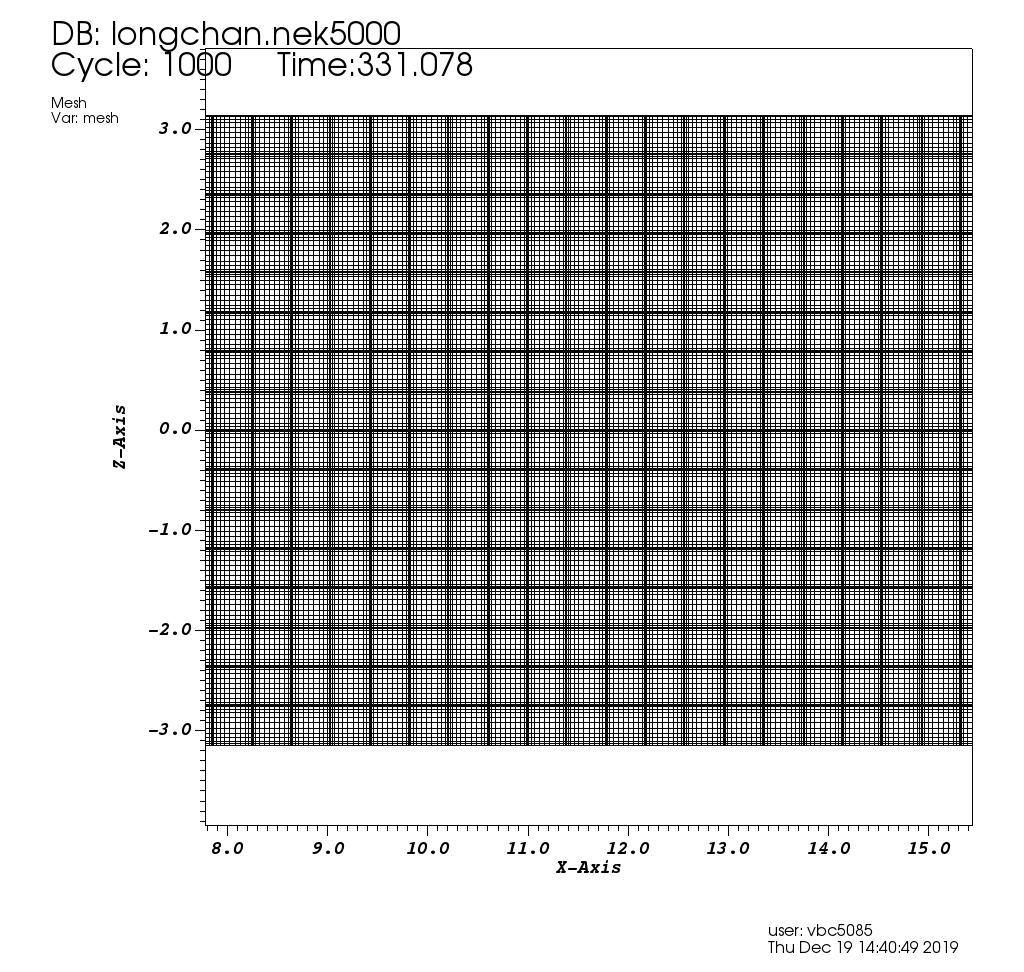
\includegraphics{mesh.png}}
	\caption{The grid employed in the simulation from half of the channel's cross section.}
	\label{fig:mesh}
\end{figure}

DNS simulations are able to simulate the finest turbulent length scales without using any turbulent model. Since the present work is focused on studying the contribution of the smaller scales to the energy cascade, it is required to use DNS rather than Reynolds 
ge Navier-Stokes (RANS) or Large Eddy Simulations (LES), although there is a substantial growth of the computational cost.

%%%%%%%%%%%%%%%%%%%%%%%%%%%%%%%%%%%%%%%%%%%%%%%%%%%%%%%%%%%%%%%%%%%%%%
\section*{METHODS - CONVOLUTION ANALYSIS OF THE FRICTION REYNOLDS NUMBER}


The friction Reynolds number has been calculated via numerical simulations for Cases I, II and III and this result was compared to the values obtained using an existed expression from Ref.~\cite{pope} valid for fully developed turbulent flows. A delay in space can be seen between \(Re_{\tau}\) when comparing the simulations' results with the values yielded from the mentioned expression. This way, these results are treated as signals in the space and a convolution operation is performed over the analytical expression for fully developed turbulent flows in order to built a function that should matches with the obtained values from the simulations.

To calculate the friction Reynolds number from the simulations several velocities profiles along \(x\) were obtained from the results and the viscous stress \(\frac{d<U>}{dy}\) for these locations are calculated. Such values can then be applied in the set of definitions given from Eqn.~\ref{shear_wall} to Eqn.~\ref{friction_reynolds} following presented in order to calculate \(Re_{\tau}\).

\begin{equation}
{\tau}_w = \rho\nu\left(\frac{d<U>}{dy}\right)_{y=0}
\label{shear_wall}
\end{equation}

Where \(\rho\) is the density and \({\tau}_w\)  is the shear stress at the wall.

\begin{equation}
u_{\tau} = \sqrt{\frac{{\tau}_w}{\rho}}
\label{u_t}
\end{equation}

Where \(u_{\tau}\) is the friction velocity. And finally,

\begin{equation}
Re_{\tau} = \frac{u_{\tau}\delta}{\nu}
\label{friction_reynolds}
\end{equation}

Where \(\delta\) is the height of the simulated channels. For all Cases studied here this is a constant parameter \(\delta=2\).

The friction Reynolds number calculated using Eqn.~\ref{friction_reynolds} with the numeric simulations' results is then compared with Eqn.~\ref{reynolds_approximation} from Ref.~\cite{pope}, which is valid for fully developed turbulent flows.

\begin{equation}
Re_{\tau} = 0.09Re^{0.88}
\label{reynolds_approximation}
\end{equation}

The Reynolds numbers used to supply Eqn.~\ref{reynolds_approximation} are those varying through \(x\) from Cases I, II and III, as presented in Fig.~\ref{fig:reynolds}. The convolution to be performed over Eqn.~\ref{reynolds_approximation} is given by Eqn.~\ref{convolution}. In this equation \(Re(\chi)\) stands for the analytical approximation given by Eqn.~\ref{reynolds_approximation}, \(g(x-\chi)\)  is a shifting function and \(\chi\) is simply a dummy variable for the streamwise distance.

\begin{equation}
F(x) =  \int_{-\infty}^{+\infty} Re_{\tau}(\chi)g(x-\chi)d\chi
\label{convolution}
\end{equation}

As mentioned earlier, the simulated channels in the present study are divided in three Regions, as shown in Fig.~\ref{fig:geometry_turbchannel}, thus, a different delayed function should be employed for each one of those. Since there is no delay in Region I, no special treatment is required for it, thus \(F(x)=Re_{\tau}(x)=550\). Differently, in Region II and III the results from the numerical experiments are delayed when compared to those from Eqn.~\ref{reynolds_approximation} and because of that a convolution operator takes place. Since we are dealing with a delayed signal in both Regions, a decaying exponential has been used as a shifting function, as proposed in Ref.~\cite{signals}.

In Region II, the friction Reynolds number is a linear function given by Eqn.~\ref{region2_reynolds}.

\begin{equation}
Re_{\tau}(x)=ax+550
\label{region2_reynolds}
\end{equation}

Where \(a\) is the linear coefficient of the increasing viscosity for each one of the three cases in Region II. Using Eqn.~\ref{region2_reynolds} in conjunction to the definition from Eqn.~\ref{convolution}, one may derive Eqn.~\ref{region2_delayed}, which is the delayed function valid for Region II of the considered Cases.

\begin{equation}
F(x)= \frac{a}{R^2}(e^{-R(x-{\delta}_{II})}-1)+\frac{a}{R}(x-{\delta}_{II})+550
\label{region2_delayed}
\end{equation}

Where \({\delta}_{II}\) is the streamwise position that Region II starts and \(R\) is named relaxing parameter and it stands for the exponential decaying constant to be used in the shifting function \(g(x-\chi)\) when dealing with Region II.

Eqn.~\ref{region3_delayed} is the delayed function yielded applying Eqn.~\ref{convolution} over Region III, where a constant friction Reynolds number \(Re_{\tau}\) predicted by Eqn.~\ref{reynolds_approximation} takes place.

\begin{equation}
F(x)= (20000-{\Lambda})(1-e^{-C(x-{\delta}_{III})})+{\Lambda}
\label{region3_delayed}
\end{equation}

In this equation \({\delta}_{III}\) is the streamwise position that Region III starts, \(C\) is named contractioning parameter and it stands for the exponential decaying constant to be used in the shifting function \(g(x-\chi)\) when dealing with Region III and finally
 \({\Lambda}=\frac{a}{R^2}(e^{-R({\delta}_{III}-{\delta}_{II})}-1)+\frac{a}{R}({\delta}_{III}-{\delta}_{II})+550\), represents the contribution from Regions II to the delayed signal in Region III.

In summary, Eqn.~\ref{delayed} express the delayed function for \(Re_{\tau}\) over different Regions of the turbulence channels considered in the present work. 

\begin{equation} \label{delayed}
F(x) = \\
    \left\{\begin{array}{@{}lr@{}}
        550  & \text{(Region I)}\\
        \frac{a}{R^2}(e^{-R(x-{\delta}_{II})}-1)+\frac{a}{R}(x-{\delta}_{II})+550 & \text{(Region II)}\\
        (20000-{\Lambda})(1-e^{-C(x-{\delta}_{III})})+{\Lambda} &  \text{(Region III)}
\end{array}\right.
\end{equation}



%%%%%%%%%%%%%%%%%%%%%%%%%%%%%%%%%%%%%%%%%%%%%%%%%%%%%%%%%%%%%%%%%%%%%%

\section*{RESULTS}

Results from the three considered Cases in the present work are shown in this section. First, a comparison between the results in Region I from Case I with an existed data from Ref~\cite{iwamoto2002} is done in order to verify the model. Then, first and second order statistics results in the close to the wall region are presented also just for Case I in the interest of brevity. Third, \(Re_{\tau}\) results and a comparison of the results with the log-law is presented. Lastly, low velocity streaks are given for \(y^+<10\) region from Case I and a discussion about these structures takes place.

\subsection*{Model verification}

In order to verify the model, results from first region in Case I, where \(Re_{\tau}=550\), were compared to existed data from Ref.~\cite{iwamoto2002}, in which DNS results of a turbulent channel with \(Re_{\tau}=650\) is found. Fig.~\ref{fig:comparing_u} shows the mean velocity \(u^+\) versus \(y^+\) plots for both results, while Fig.~\ref{fig:comparing_uu} shows the Reynolds stress \(<uu>\) versus \(y^+\) plots. These graphs shows that the results from both simulations follows the expected behaviour, this fact grants confidence to the models used in the present work.

\begin{figure}[t]
\centering
\scalebox{0.5}
{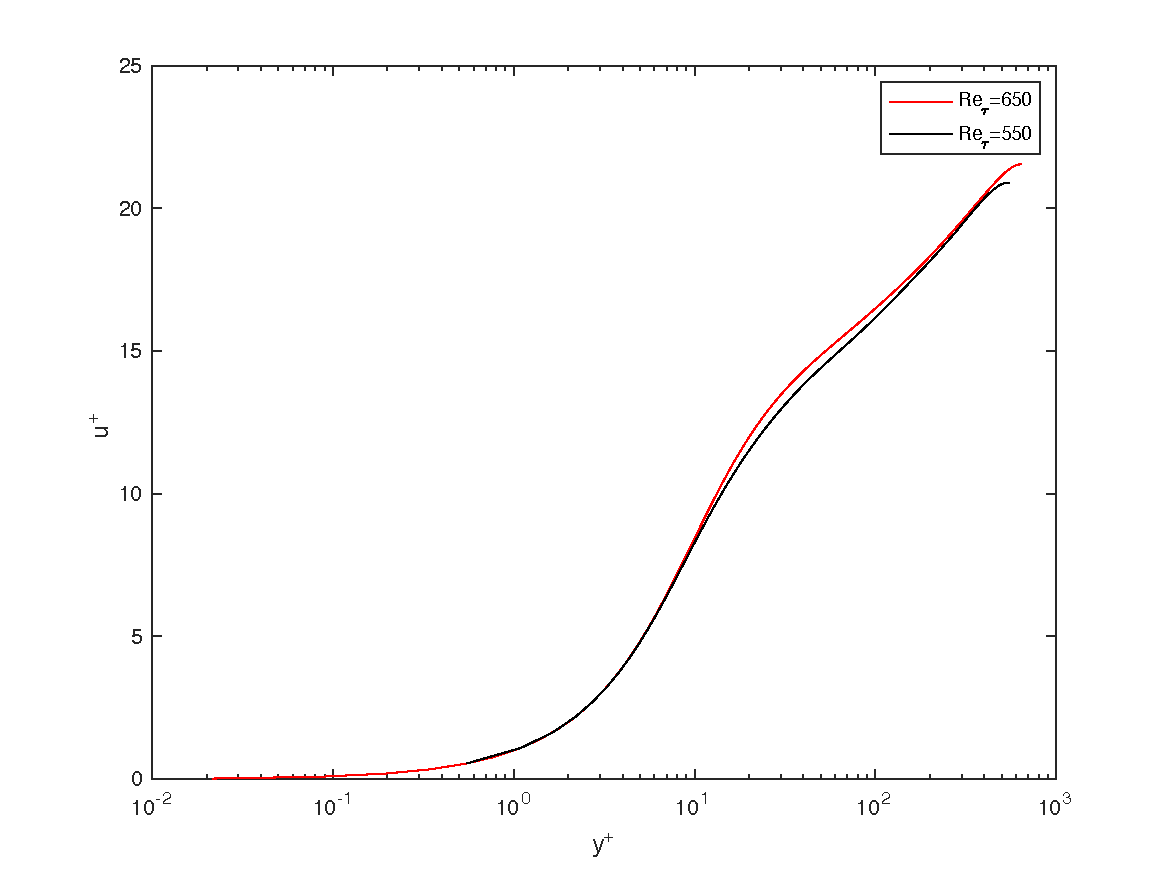
\includegraphics{comparing_u.pdf}}
\caption{Comparing \(u^+\) from Region I in Case I, where \(Re_{\tau}=550\), with already existed data from Ref.~\cite{iwamoto2002}, where \(Re_{\tau}=650\).}
\label{fig:comparing_u}
\end{figure}

\begin{figure}[t]
\centering
\scalebox{0.5}
{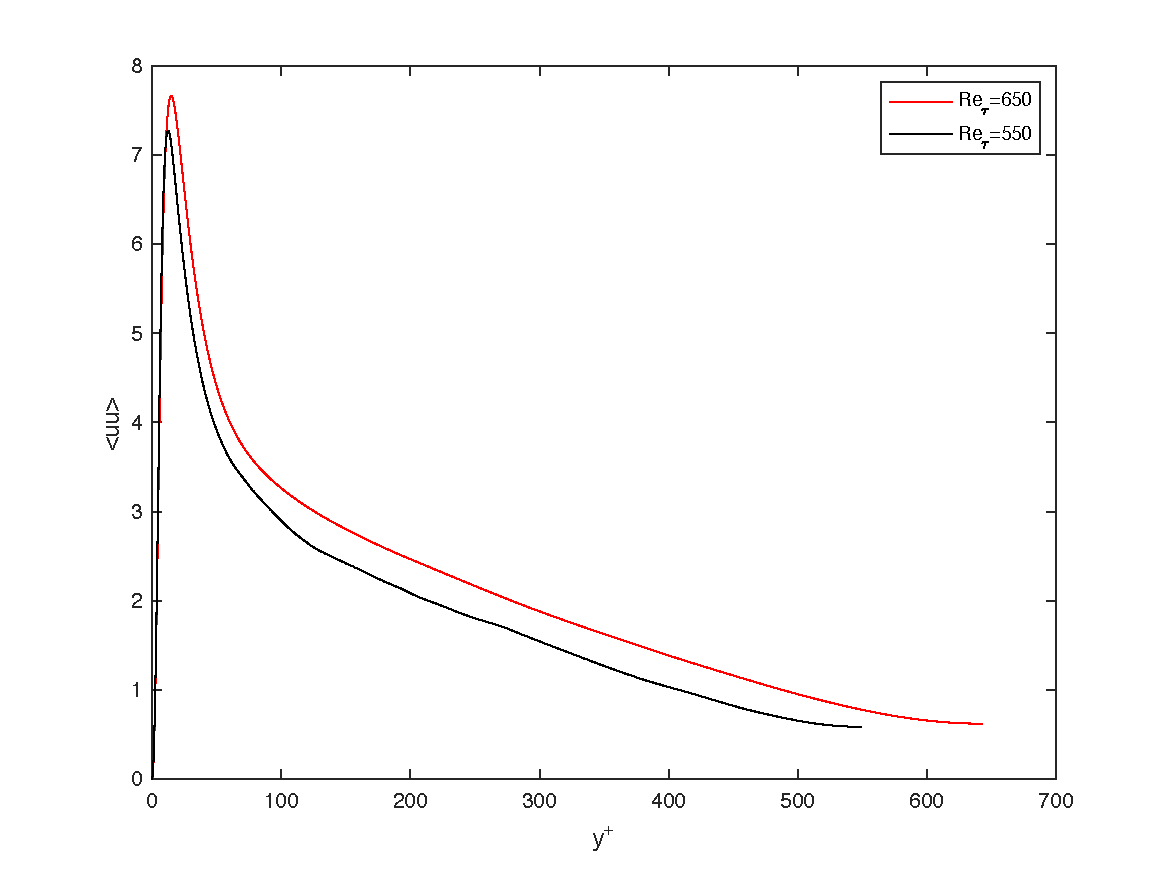
\includegraphics{comparing_uu.pdf}}
\caption{Comparing \(<uu>\) from Region I in Case I, where \(Re_{\tau}=550\), with already existed data from Ref.~\cite{iwamoto2002}, where \(Re_{\tau}=650\).}
\label{fig:comparing_uu}
\end{figure}

\subsection*{First and second order statistics}

The averaging time employed to obtain statistics results for Case I was judged sufficient since it allowed the solution to reach near perfect symmetry. Furthermore, to reduce this time spatial average has been taken over the spanwise direction, since the flow is homogeneous in this direction.

Fig.~\ref{fig:u_CI}  shows how \(<u>\) profile develops along the channel in Case I. From this result we can clearly see that the viscous stress at the wall \(\left(\frac{d<U>}{dy}\right)_{y=0}\) gets more pronounced as we move in the streamwise direction. This result makes sense, since in Region II the viscosity starts decreasing linearly, as shown through Fig.~\ref{fig:viscosity}, causing the viscous effects to become more pronouced. This fact also explains why the turbulent boundary layer \((y^+=30)\) starts getting closer to the wall in this same range, fact also presented in Fig.~\ref{fig:u_CI}. Moreover, after a certain value of \(x\), the boudary layer reaches a constant height from the wall, this fact also makes sense once in Region III the viscosity becomes constant, not causing a change in the viscous stress anymore.

\begin{figure}[t]
\centering
\scalebox{0.5}
{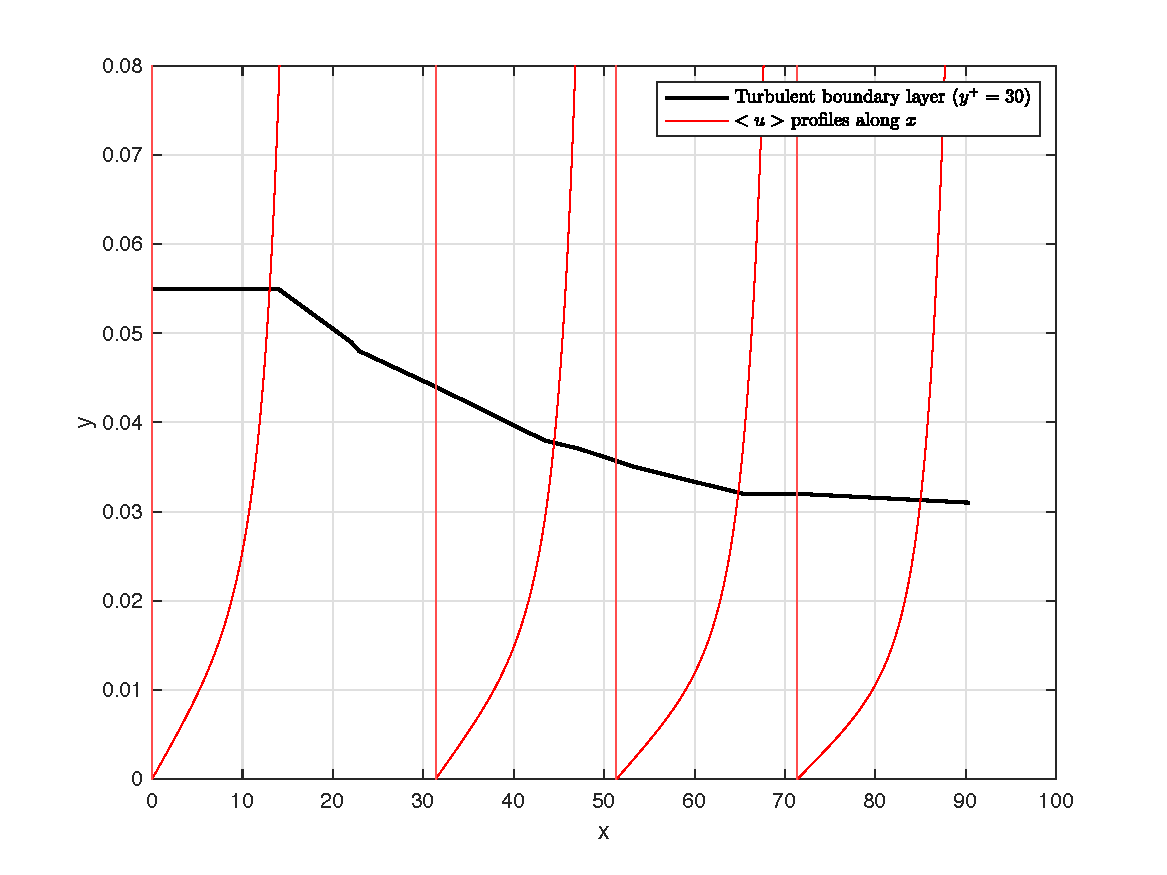
\includegraphics{u_CI.pdf}}
\caption{Mean velocity \(<u>\) profiles along the streamwise direction and the turbulent boudary layer \((y^+=30)\).}
\label{fig:u_CI}
\end{figure}

Fig.~\ref{fig:uu_CI} shows \(<uu>\) profile development throughtout the streamwise direction also for Case I. As we move foward in the streamwise direction in this plot, the peak of \(<uu>\) increases and gets closer to the wall. This result is also in good agreement with what is expected, since the turbulence must increase in Region II.

\begin{figure}[t]
\centering
\scalebox{0.5}
{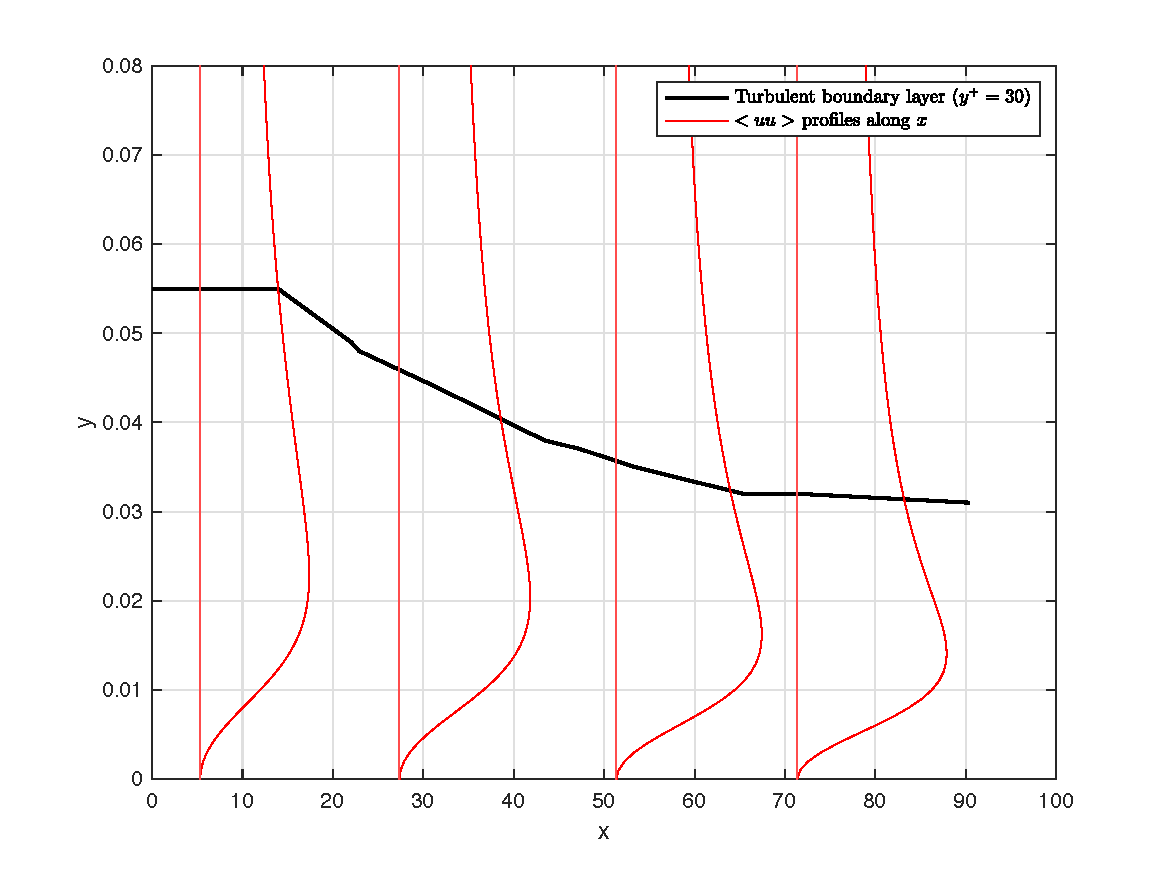
\includegraphics{uu_CI.pdf}}
\caption{Reynolds stress \(<uu>\) profiles along the streamwise direction and the turbulent boudary layer (\(y^+=30)\).}
\label{fig:uu_CI}
\end{figure}

\subsection*{Delayed friction Reynolds number}

In practice terms, Eqn.~\ref{delayed} delays the signal resulted from the appoximation given by Eqn.~\ref{reynolds_approximation}. This is true once the former expression is the result of a convolution operation over the last one. One might notice that Eqn.~\ref{delayed} dependes on two parameters, i.e., the contractioning parameter \(C\) and the relaxing parameter \(R\), this way, a suitable method for measuring how much delayed is the \(Re_{\tau}\) when varying the viscosity from a fully developed turbulent condition is by adjusting these parameters so that the delayed function \(F(x)\) well fitted the simulated results.

The abovementioned procedure has been performed for Cases I, II and III considered in the present work. Figs.~\ref{fig:convolution_CI}-\ref{fig:convolution_CIII} refers to the friction Reynolds resulted from these simulations respectively. In each one of these plots the parameters \(C\) and \(R\) were calibrated so the delayed function fits in the simulated results. The estimated values for these two parameters are \(C=1.162\) and \(R=0.030\). One should notice that these values kept the same regardless how fast the viscosity changes along \(x\).

\begin{figure}[t]
\centering
\scalebox{0.4}
{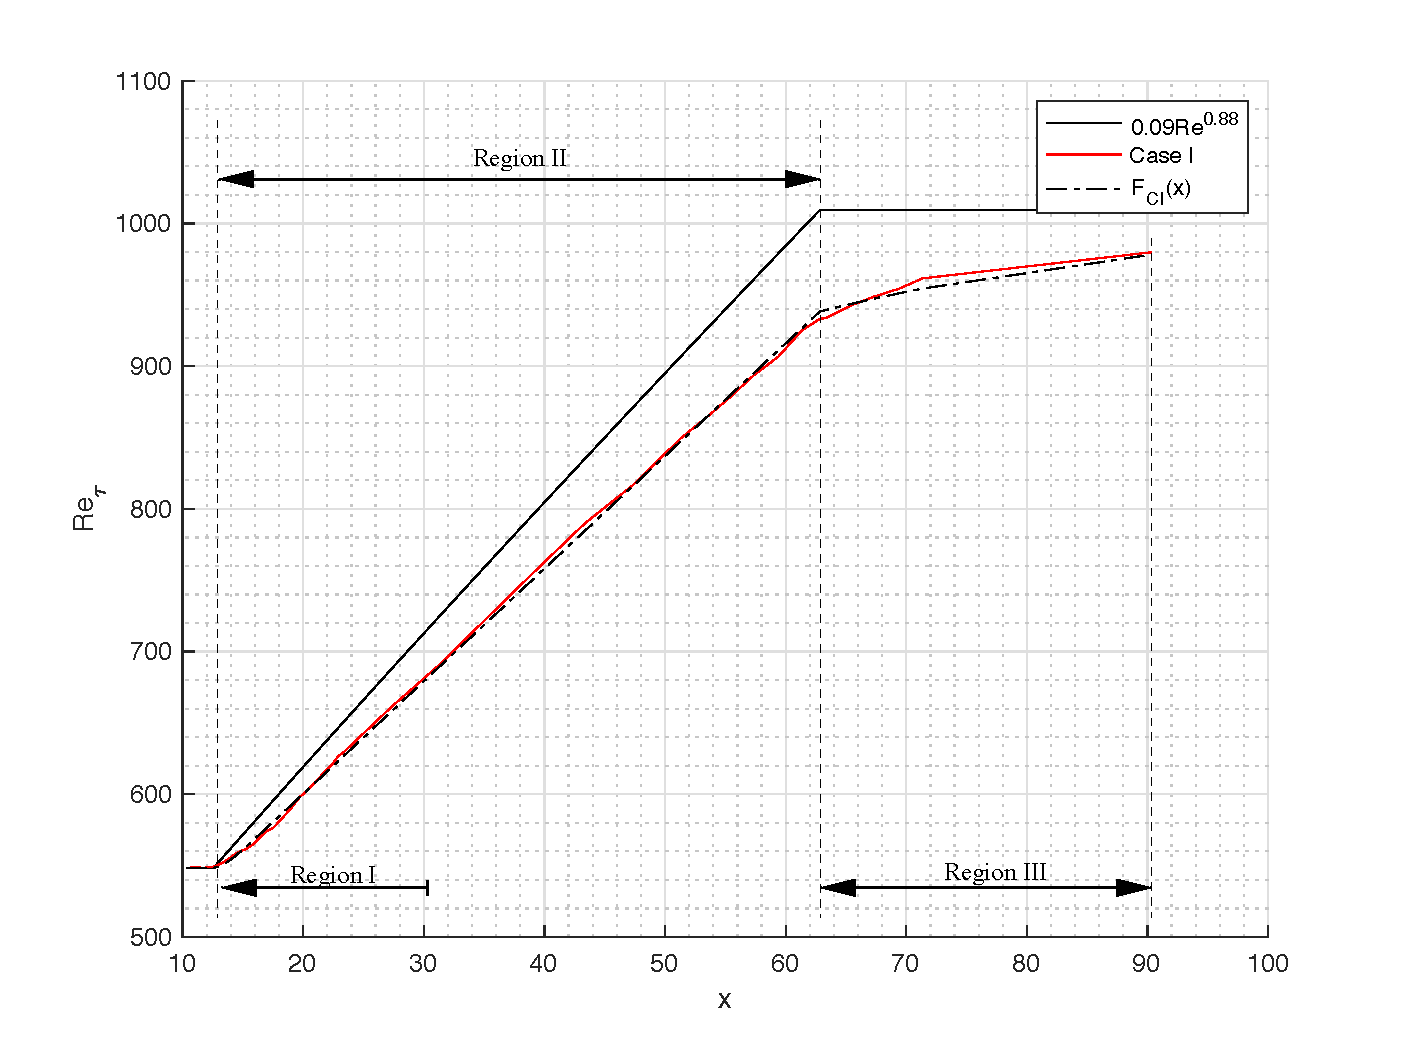
\includegraphics{convolution_CI.pdf}}
\caption{Friction Reynolds number through \(x\) for Case I.}
\label{fig:convolution_CI}
\end{figure}

\begin{figure}[t]
\centering
\scalebox{0.4}
{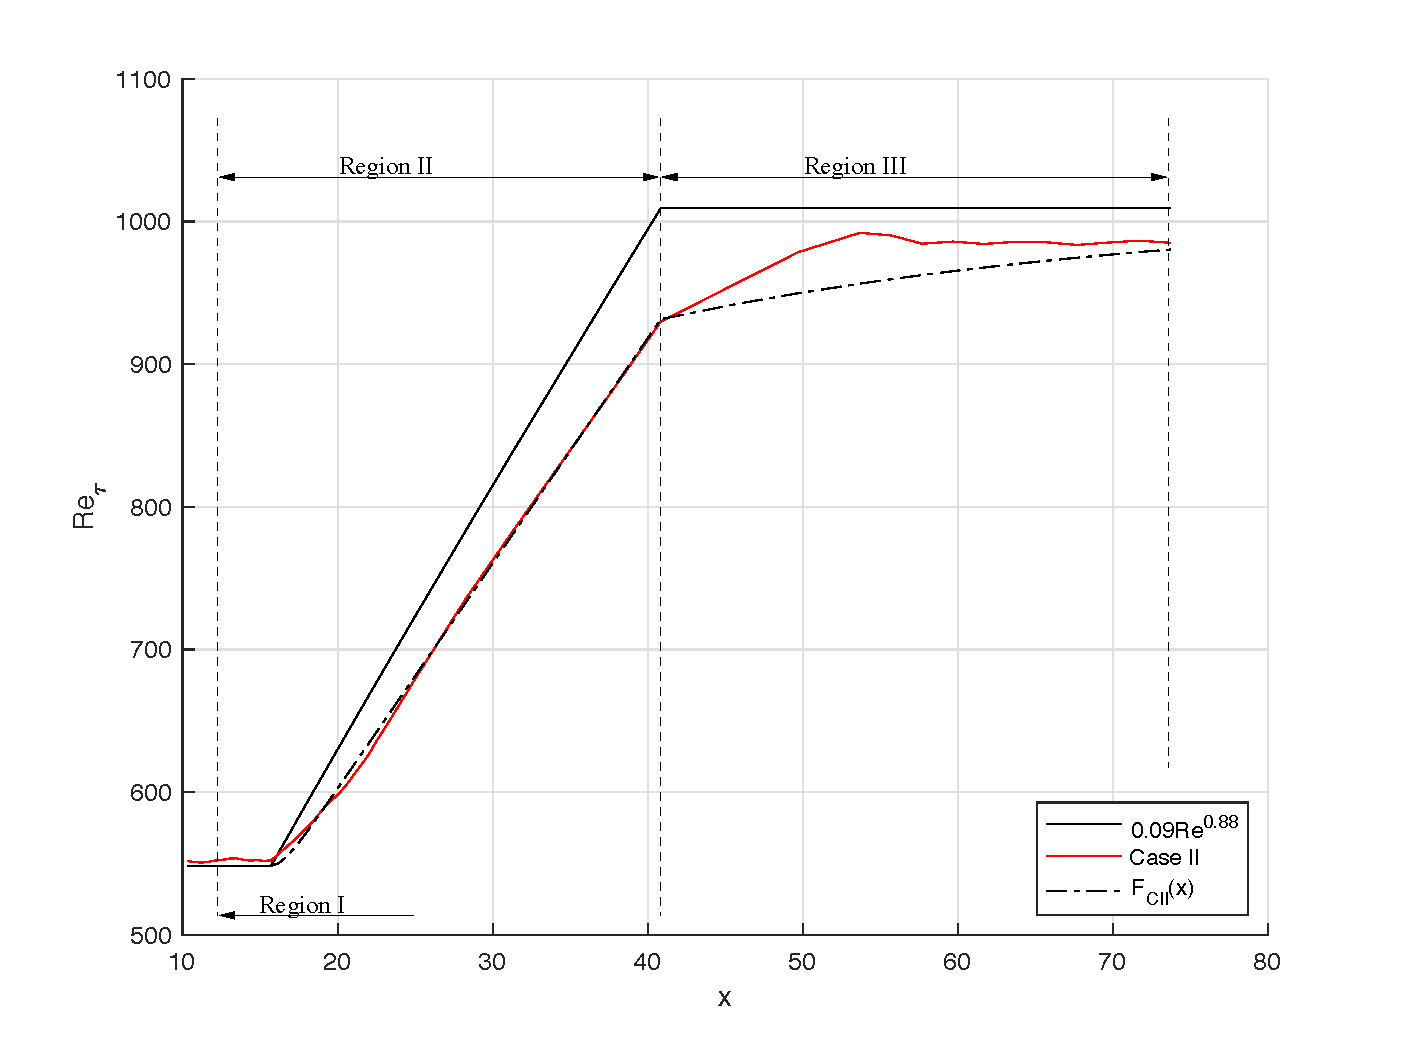
\includegraphics{convolution_CII.pdf}}
\caption{Friction Reynolds number through \(x\) for Case II.}
\label{fig:convolution_CII}
\end{figure}

\begin{figure}[t]
\centering
\scalebox{0.4}
{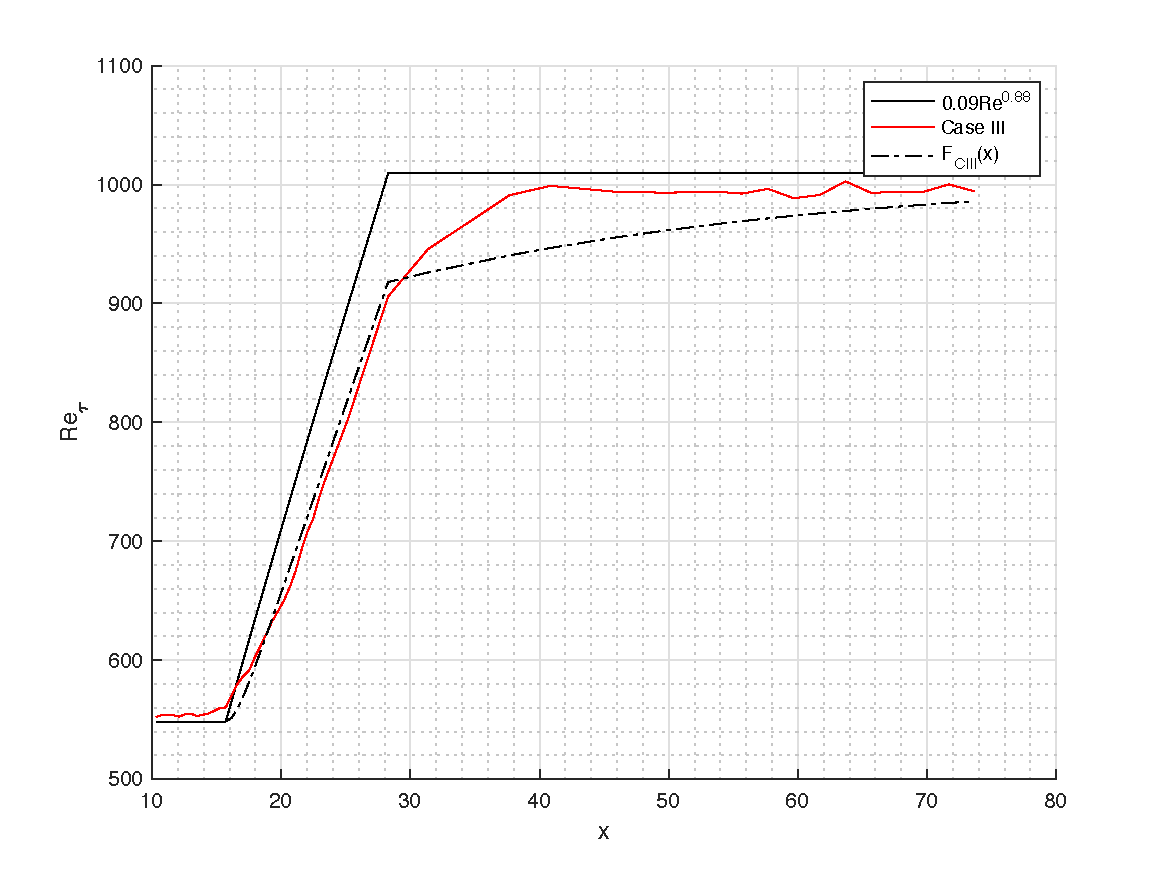
\includegraphics{convolution_CIII.pdf}}
\caption{Friction Reynolds number through \(x\) for Case III.}
\label{fig:convolution_CIII}
\end{figure}

Unfourtunantly, it was not possible to run Cases II and III for the same long as Case I, thus the results for these simulations did not reach statistically stability. However, it seems that the results of these simulations are approaching to the same values provided by the delay function so far employed.

Fig.~\ref{fig:log_law_CI_upstream} and Fig.~\ref{fig:log_law_CI_downstream} shows a comparison between the mean velocity profile \(u^+\) versus \(y^+\) from Case I and the log-law at different locations along \(x\).

In Fig.~\ref{fig:log_law_CI_upstream} we can see that the \(u^+\) profile is in good agreement with the log-law at \(x=4{\pi}\), however, isofar we move in the downstream direction, the profile stops following the log-law, which is the case of the profiles at \(x=12{\pi}\) and at \(x=20{\pi}\), where it gets even more off. The increasing lack of agreement with the log-law means that the flow is becoming less developed at these locations throughout Region II. This fact is closely related to what is observed in the graph from Fig.~\ref{fig:convolution_CI} in the sense that as \(Re_{\tau}\) from Case I is more delayed in space when comparison to a fully developed flow it has less agreement with the log-law. This fact becomes more clear when analysing \(x=20{\pi}\) profile, it is noticed that this is the location where both \(Re_{\tau}\)'s delay and lack of agreement with the log-law are maximized.

Differently, in Fig.~\ref{fig:log_law_CI_downstream} the opposite trend is observed, i.e., as we move in the downstream direction throughout Region III, the \(u^+\) profile tends to become more close to the log-law. This is the expected behaviour since in this Region the viscosity is constant, thus the turbulent flow is not prevented from developing anymore. Once again, this fact is closely related to what is observed in Fig.~\ref{fig:convolution_CI}, once for Region III, \(Re_{\tau}\) from Case I starts getting less delayed in space when compared to a fully developed turbulent flow.

\begin{figure}[t]
\centering
\scalebox{0.5}
{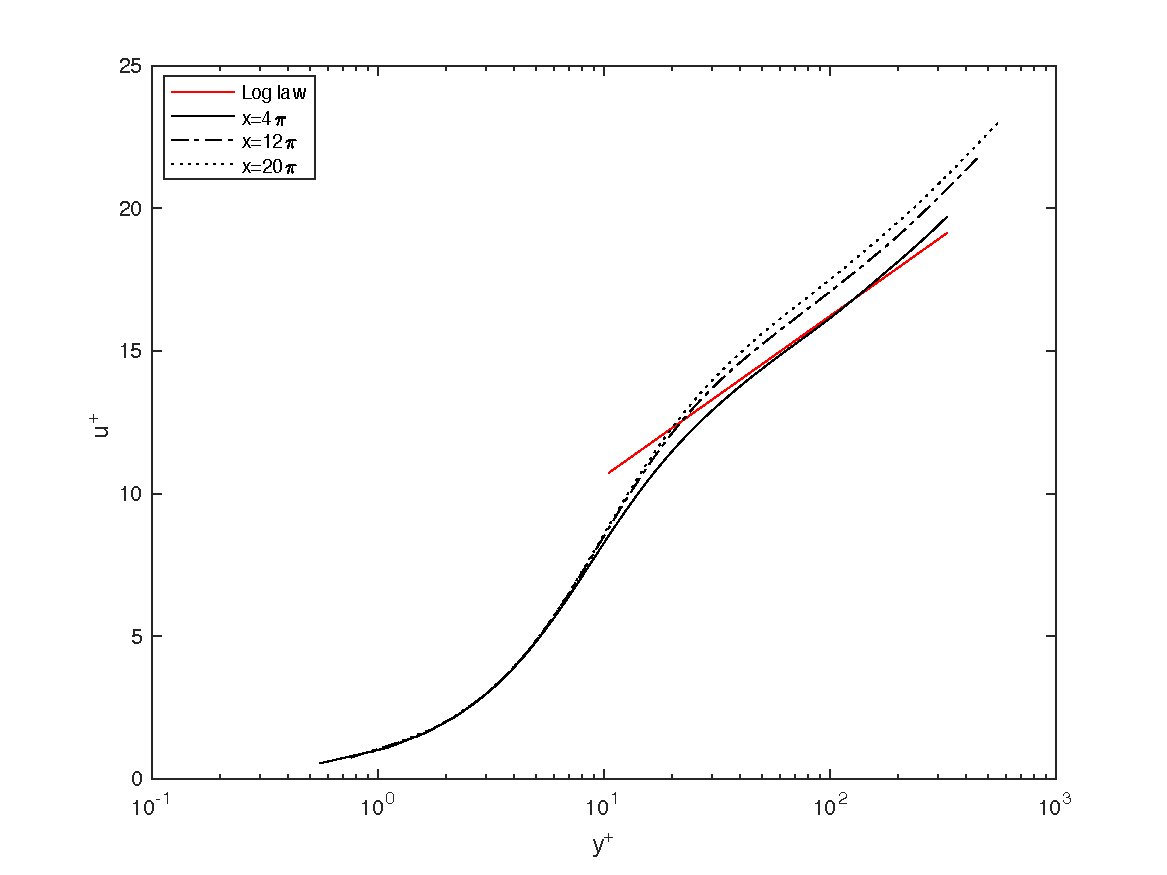
\includegraphics{log_law_CI_upstream.pdf}}
\caption{\(u^+\) versus \(y^+\) obtained from Case I at \(x=4{\pi}\) (end of Region I), \(x=12{\pi}\) (middle of Region II) and \(x=20{\pi}\) (end of Region II) compared to the log law.}
\label{fig:log_law_CI_upstream}
\end{figure}

\begin{figure}[t]
\centering
\scalebox{0.5}
{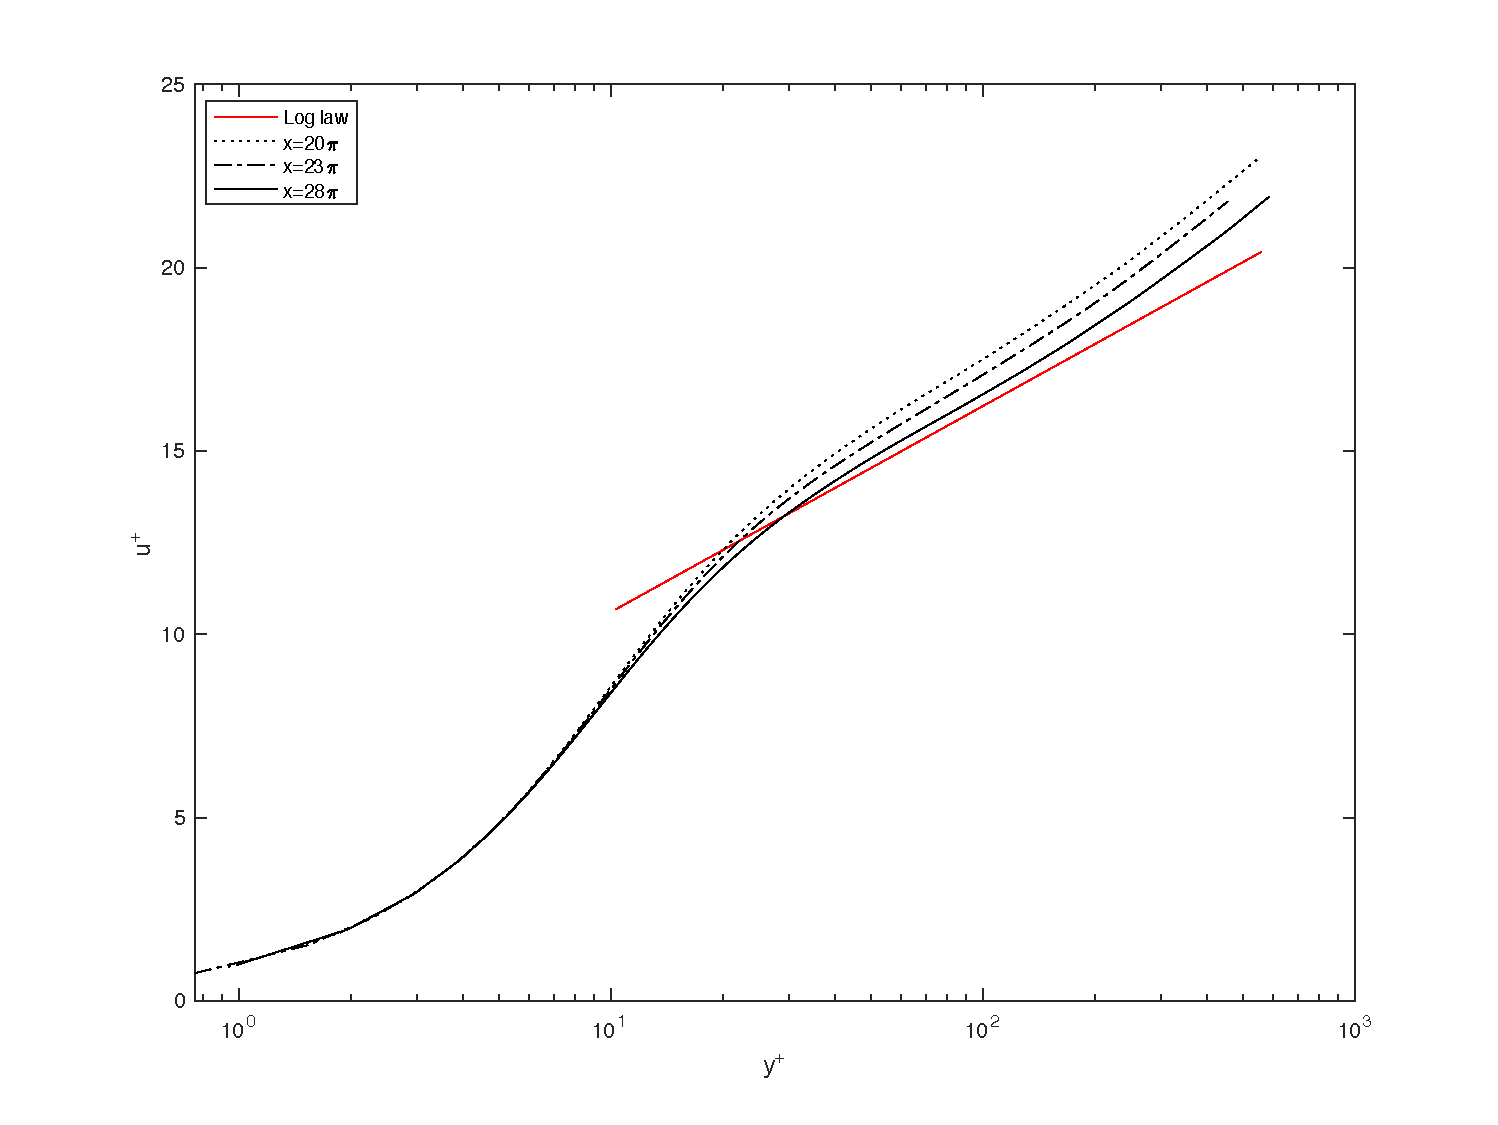
\includegraphics{log_law_CI_downstream.pdf}}
\caption{\(u^+\) versus \(y^+\) obtained from Case I at \(x=20{\pi}\) (end of Region I), \(x=23{\pi}\) (Region III) and \(x=28{\pi}\) (Region III) compared to the log law.}
\label{fig:log_law_CI_downstream}
\end{figure}

\subsection*{Turbulent structures}

Fig.~\ref{fig:streaks} has been taken from the instantaneous streamwise velocity scalar field at a height \(y=0.01\) from the wall. Low-velocities streaks are allowed to be visualized by employing convinient pseudocolor thresholds. Through visual verification, it is possible to measure that the lenght of these structures varies in a range of \(500\) to \(2000\) wall units, which is consistent with the literature Ref.~\cite{carlier2005}. Furthermore, it is also noticed that the streaks' length does not change along the streamwise direction. However, the distance separating one from the other in the transverse direction, i.e., the spanwise direction, notably increases.

Two-points correlation in the spanwise direction has been performed correlating the streamwise direction velocities for the present work. This measures has been taken over different positions in the turbulent channel in Case I, Fig.~\ref{fig:spanwise_correlation} shows these results. One may notice that as we move foward in \(x\) the correlation of the measured signals becomes more strong. The increasing correlation in the measure is actually due to what is noticed from the streaks showed in Fig.~\ref{fig:streaks}, i.e., these structures becomes more separated as we move in the downstream portion of the channel.

\begin{figure*}[t]
	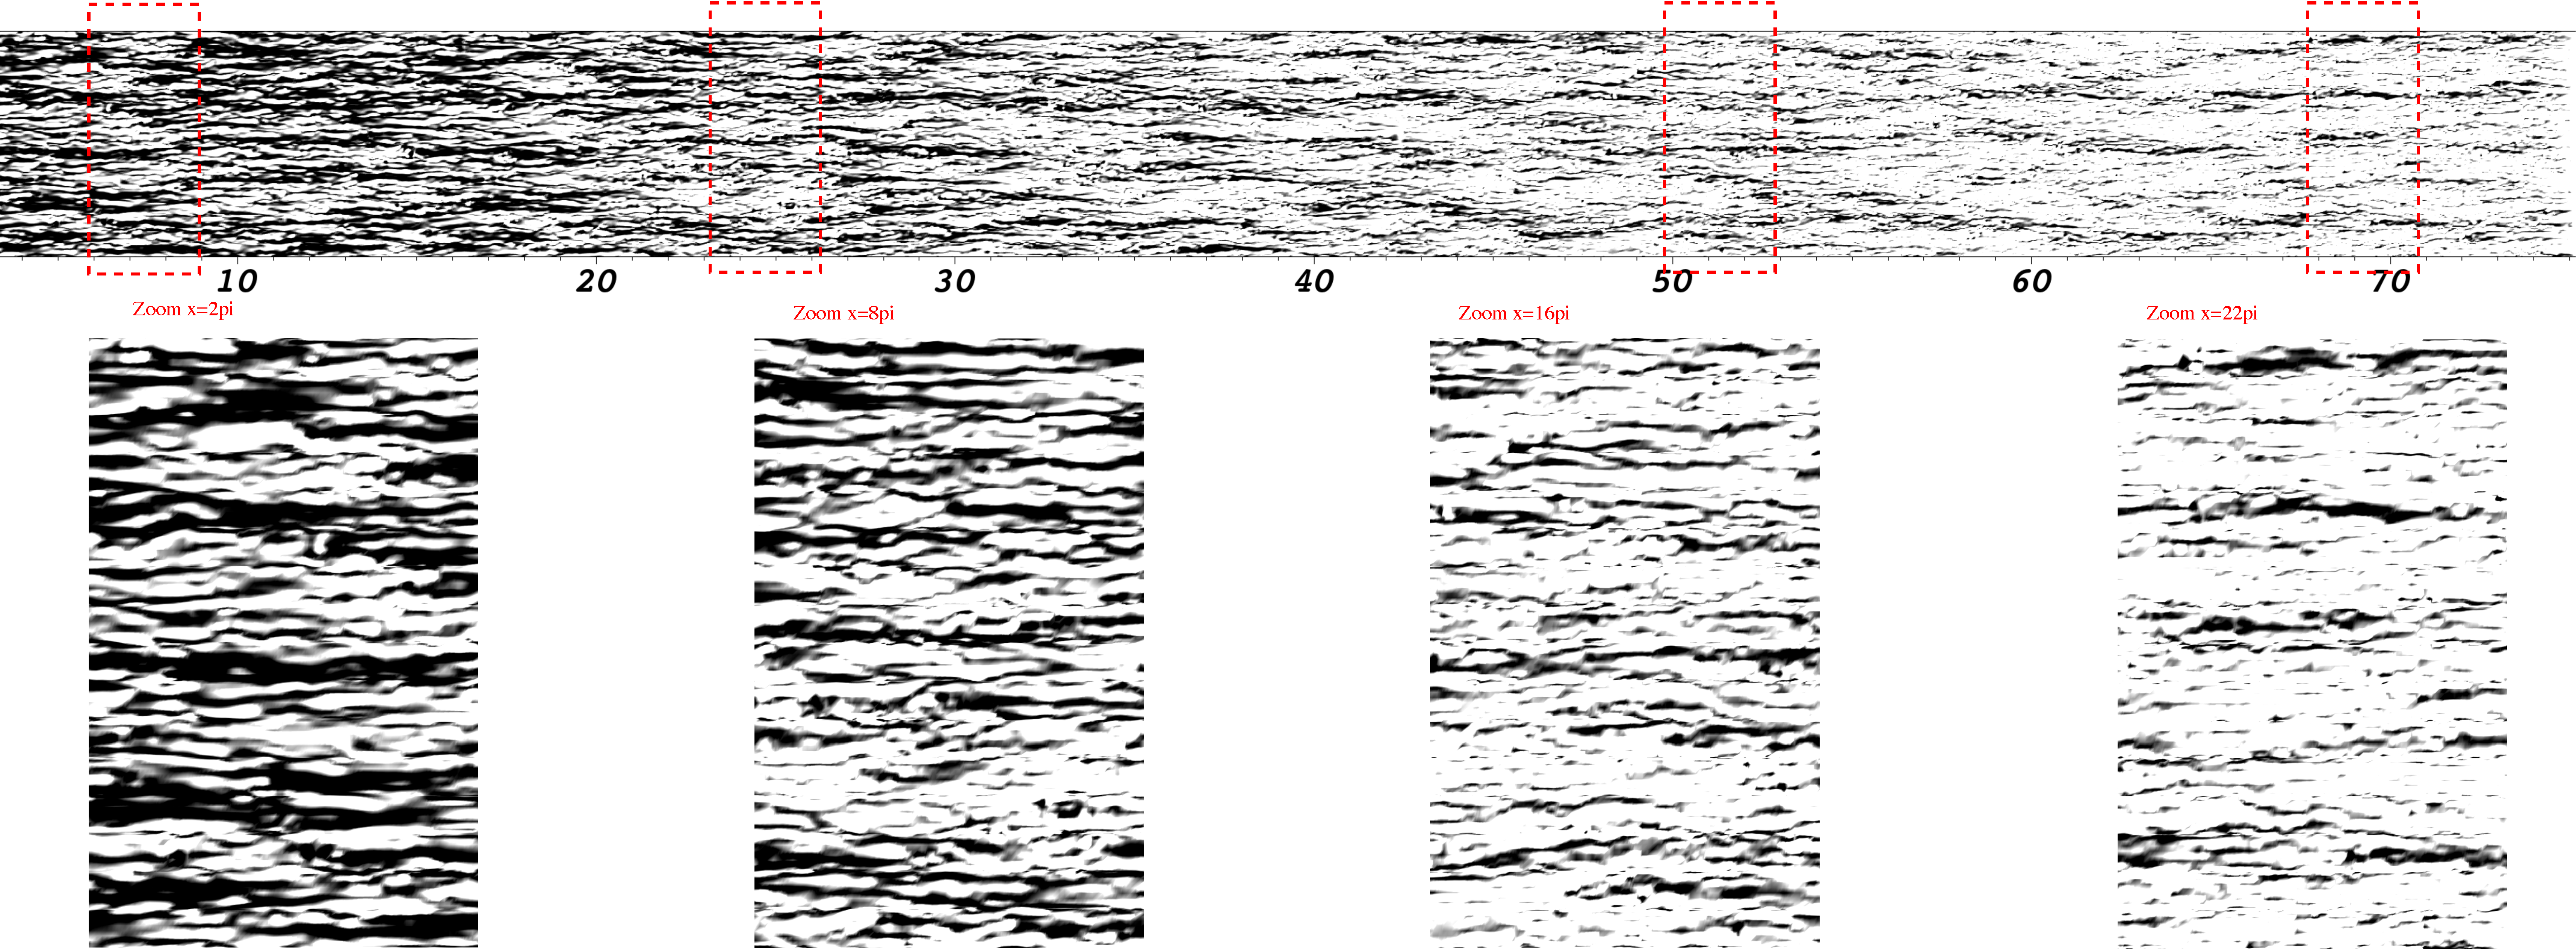
\includegraphics[width=\textwidth]{streaks.pdf}
	\caption{A cross section of the instantaneous streamwise velocity field at 0.01 from the wall.}
	\label{fig:streaks}
\end{figure*}

\begin{figure}[t]
\centering
\scalebox{0.5}
{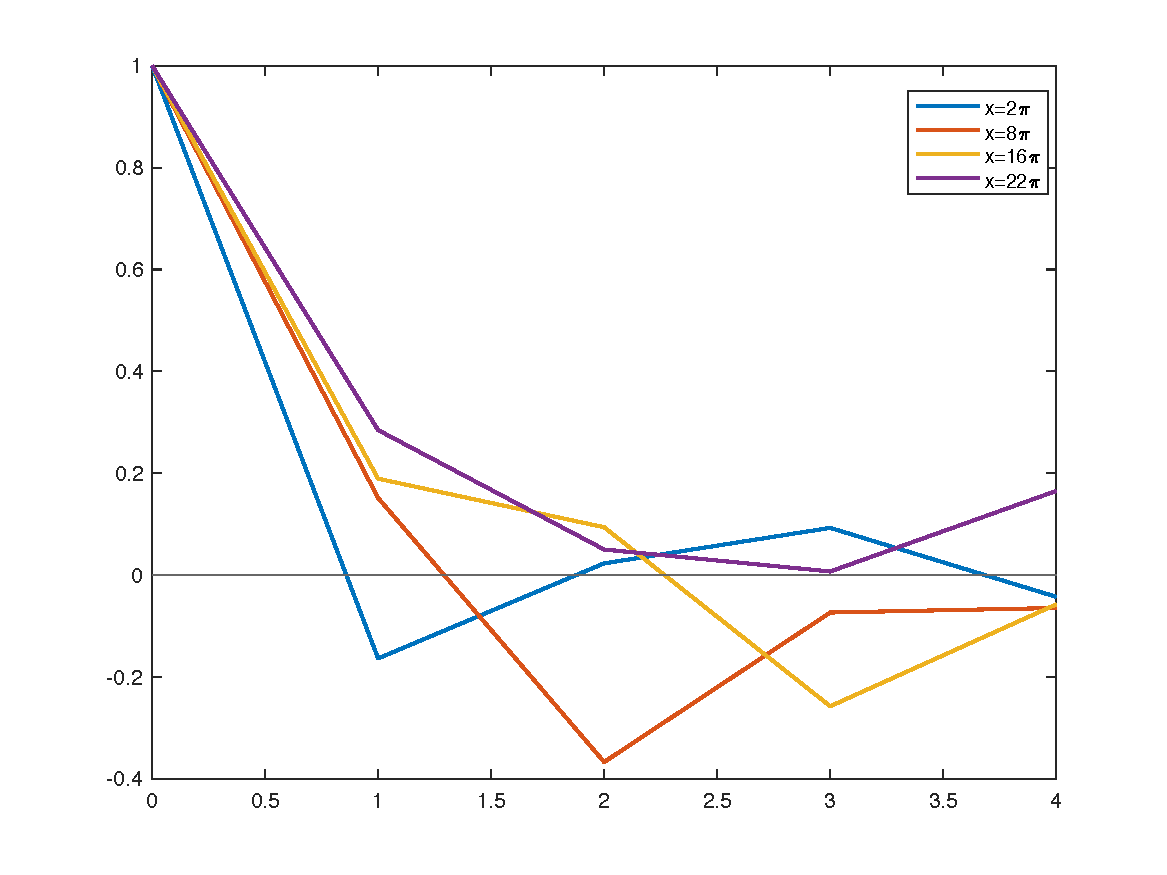
\includegraphics{spanwise_correlation.pdf}}
\caption{Two-point correlation of \(u\) over the spanwise direction at different streamwise distances.}
\label{fig:spanwise_correlation}
\end{figure}

%%%%%%%%%%%%%%%%%%%%%%%%%%%%%%%%%%%%%%%%%%%%%%%%%%%%%%%%%%%%%%%%%%%%%%
\section*{CONCLUSIONS}


%%%%%%%%%%%%%%%%%%%%%%%%%%%%%%%%%%%%%%%%%%%%%%%%%%%%%%%%%%%%%%%%%%%%%%
\begin{acknowledgment}
Thanks go to D. E. Knuth and L. Lamport for developing the wonderful word processing software packages \TeX\ and \LaTeX. I also would like to thank Ken Sprott, Kirk van Katwyk, and Matt Campbell for fixing bugs in the ASME style file \verb+asme2e.cls+, and Geoff Shiflett for creating 
ASME bibliography stype file \verb+asmems4.bst+.
\end{acknowledgment}

\bibliographystyle{asmems4}

\bibliography{asme2e}
\appendix   

\end{document}
